\documentclass{vldb}
\usepackage{balance}
\usepackage[utf8]{inputenc}
\usepackage[T1]{fontenc}
\usepackage[english]{babel}
\usepackage[activate={true,nocompatibility},final,kerning=true,spacing=true,factor=1100,stretch=10,shrink=10]{microtype}
\usepackage[subtle]{savetrees}
\usepackage{amsfonts,amssymb,amsmath}
\usepackage{xcolor}
\usepackage{algorithm}
\usepackage[noend]{algpseudocode}
\usepackage[style=numeric,firstinits=true]{biblatex}
\usepackage{booktabs}
\usepackage{siunitx}
\usepackage{graphicx} % includegraphics
\usepackage{listings} % code samples with syntax hl
\usepackage{stmaryrd}
\usepackage{qtree} % for simple tree diagrams
\usepackage{caption}
\usepackage{subcaption}
\usepackage{xcolor}
\usepackage{hyperref} % load after other packages
\usepackage{tikz}
\usetikzlibrary{positioning}
\usepackage{cleveref}
\usepackage{xspace}

\newcommand{\srm}[1]{\textcolor{red}{SAM:#1}}
\addbibresource{references.bib}

\renewcommand{\algorithmicrequire}{\textbf{Input:}}
\renewcommand{\algorithmicensure}{\textbf{Output:}}

% listings settings
\lstset{ %
  backgroundcolor=\color{white},   % choose the background color; you must add \usepackage{color} or \usepackage{xcolor}; should come as last argument
  basicstyle=\ttfamily\footnotesize,        % the size of the fonts that are used for the code
  breakatwhitespace=false,         % sets if automatic breaks should only happen at whitespace
  breaklines=true,                 % sets automatic line breaking
  captionpos=b,                    % sets the caption-position to bottom
  commentstyle=\color{red},    % comment style
  %frame=single,	                   % adds a frame around the code
  keepspaces=true,                 % keeps spaces in text, useful for keeping indentation of code (possibly needs columns=flexible)
  keywordstyle=\color{blue},       % keyword style
%  numbers=left,                    % where to put the line-numbers; possible values are (none, left, right)
  numbersep=5pt,                   % how far the line-numbers are from the code
%  numberstyle=\tiny\color{gray}, % the style that is used for the line-numbers
  rulecolor=\color{black},         % if not set, the frame-color may be changed on line-breaks within not-black text (e.g. comments (green here))
%  stepnumber=2,                    % the step between two line-numbers. If it's 1, each line will be numbered
  stringstyle=\color{red},     % string literal style
  tabsize=2,	                   % sets default tabsize to 2 spaces
  language=SQL
}

\makeatletter
\newcommand*{\centerfloat}{%
  \parindent \z@
  \leftskip \z@ \@plus 1fil \@minus \textwidth
  \rightskip\leftskip
  \parfillskip \z@skip}
\makeatother

\DeclareMathOperator*{\argmax}{arg\,max}
\DeclareMathOperator*{\argmin}{arg\,min}

\MakeRobust{\Call}

\renewcommand{\emptyset}{\varnothing}

\newcommand{\ProjectName}{ImputeDB\xspace}
\newcommand{\sys}{\ProjectName}
\newcommand{\doms}[2]{#1 \succ #2}

% definitions/theorems etc
\newtheorem{definition}{Definition}
\newtheorem{theorem}{Theorem}
\newtheorem{case}{Case}

% new section names for cref
\Crefname{query}{Query}{Query}

\title{\ProjectName{}: Data Imputation as a Query Optimization}

\author{
  Jos\'e Cambronero \\
  \texttt{jcamsan@csail.mit.edu}
  \and
  John K. Feser \\
  \texttt{feser@csail.mit.edu}
  \and
  Micah J. Smith \\
  \texttt{micahs@mit.edu}}

\newcommand{\fix}{\marginpar{FIX}}
\newcommand{\new}{\marginpar{NEW}}
\newcommand{\todo}[1]{{\color{red}\textbf{TODO:} #1}}
\newcommand{\todobox}[2]{{\color{red}\fbox{\parbox{\columnwidth}{\textbf{TODO:} #1\\#2}}}}

% results that can be used in any section
\newcommand{\demorows}{10175}
\newcommand{\labexrows}{9813}
\newcommand{\acsbaseresultminutes}{355 minutes}
\newcommand{\acsbaseresulthours}{just under 6 hours}
\newcommand{\acsimputedbzeroresult}{4 seconds}
\newcommand{\acsimputedboneresult}{1 second}
\newcommand{\lowxalphazero}{10}
\newcommand{\lowsmapealphazero}{0}
\newcommand{\highxalphaoneexacs}{1000}
\newcommand{\highsmapealphaoneexacs}{24}
\newcommand{\highxalphaone}{16000}

\begin{document}

\maketitle

\begin{abstract}
Missing values abound in data analysis and often present a serious challenge for usability of data. Users
are forced to pick between removing tuples with missing values or creating a clean duplicate of their data
by  applying a potentially-expensive imputation strategy. We show that it is possible
to incorporate imputation into a cost-based query optimizer, performing imputation on the fly
for each query. This allows users to immediately explore
their data, while the system picks the optimal placement of imputation operations. This placement is based
on the specific query issued and a user-provided parameter that trades off data
quality and runtime performance. We incorporate the imputation operators into the relational algebra, allowing
for traditional optimizations to take place. Our experiments evaluate this approach on two real-world survey-based datasets
from the \textit{Center for Disease Control and Prevention} and \textit{freeCodeCamp}. Our results show that the optimizer
generates query plans that execute between \lowxalphazero{} and \highxalphaoneexacs{} times as fast as imputing at the base
tables and then executing queries, making exploratory data analysis using our system feasible. Furthermore, we show that the query results
from on-the-fly imputation have Symmetric-Mean-Absolute-Percentage-Error between \lowsmapealphazero{} and \highsmapealphaoneexacs{} percent
when compared to standard full-table imputation approach.
\end{abstract}

\section{Introduction}

Many databases have large numbers of missing or \nullv{} values;  these can arise for a variety of reasons, including missing source data (e.g., unknown facts),
missing columns during data integration, de-normalized databases, or as a result of outlier detection and cleaning where \nullv{} values are substituted for
bad values~\cite{kim2003}.  Such \nullv{} values can lead to incorrect or ill-defined query results~\cite{rubin1976}, and as such removing these values from data
before processing is often desirable.

% Solution
One common approach is to manually replace missing values using a statistical or predictive model based on other values in the table and record.
This process is called \emph{imputation}.
In this paper, we introduce \ProjectName{}, a new system designed to selectively apply imputation to a subset of records, on-the-fly, during query execution.  \emph{The key insight behind \ProjectName{} is that imputation
only needs to be performed on the data relevant to a particular query and
that this subset is generally much smaller than the entire database.}  
% Background
While traditional imputation methods work over the entire data set and replace all missing
values, running a sophisticated imputation algorithm over a large data set can be very
expensive: our experiments show that even a relatively simple decision tree algorithm takes \acsbaseresulthours{} to train and run
on a 600K row database.

A simpler approach might drop all rows with missing values, which can not only introduce
bias into the results, but also result in discarding much of the data.
In contrast to existing systems~\cite{burgette2010multiple,akande2015empirical}, \ProjectName{} avoids imputing over the entire data set. Specifically, \ProjectName{}
carefully plans the placement of imputation/row-drop operations inside the query plan, resulting in a 
significant speedup in query execution while reducing the number of dropped rows. Unlike previous work, the focus of our work is not on the imputation algorithms themselves (we can employ almost any such algorithm), but rather on placing imputation operations
optimally in query plans.   Specifically, our optimization algorithms generate the
Pareto-optimal frontier of plans that trade imputation cost for result quality,
and allow the analyst to specify their desired plan from this frontier.

% \todobox{find appropriate location for this}
% {In a previous project, she
% worked with the American Community Survey data (671,153 rows), and performing imputation on the whole
% dataset took around 75 minutes\todo{Here, we can reference the number from our own experiment (done), or the number from Akande et al: ``performing imputation on just a 1.5 percent random sample took 45 minutes''}.}

% % Prior work
% There is relevant prior work in three broad areas: statistics, databases, and time-series forecasting.
% Prior work in statistics\todo{add more specific subarea qualifier} has focused on imputation quality~\cite{burgette2010multiple} and runtime cost~\cite{akande2015empirical}.
% Prior work in databases has established simple semantics for handling tuples with missing values~\cite{codd1973understanding,grant1977null}.
% Prior work in time-series forecasting has incorporated forecasting extensions into domain-specific databases and characterized their behavior~\cite{parisi2011embedding,parisi2013temporal,duan2007processing}.
% \ProjectName{} contributes the first optimizer to plan data imputation on a per query basis, allowing users to use standard SQL on real-world data sets with missing values
% and express preferences in quality of data imputation versus running time. The guiding design principle behind \ProjectName{} is that the user should never see missing data or have to modify their queries to account for it.

% Implications
Our approach enables an exploratory analysis workflow in which the analyst can issue
standard SQL queries over a data set, even if that data has missing values.
These queries execute between \lowxalphazero{} and \highxalphazeroexacs{} times as fast as it takes to impute all missing values and then run queries (the traditional approach). Furthermore, the results obtained with this approach
are similar in quality to those obtained with the traditional imputation approach
--- between \lowsmapealphazero{} and \highsmapealphaoneexacs{}
percent, in one error measure --- in our empirical results over real-world data sets (see~\Cref{sec:experiments}
for details).


\subsection{Contributions}
\ProjectName{} is designed to enable early data exploration, by allowing analysts to run
their queries without an explicit base-table imputation step. To do so, it leverages a number of contributions
to minimize imputation time while producing comparable results to traditional approaches.

These contributions include:
\begin{itemize}
\item \textbf{Relational algebra extended with imputation:}
  We extend the standard relational algebra with two new operators to represent imputation operations: impute ($\mu$) and drop ($\delta$).
  The \textit{Impute} operation fills in missing data values using any statistical imputation
  technique, such as chained-equation decision trees ~\cite{burgette2010multiple}.
  The \textit{Drop} operation simply drops tuples which contain \nullv{} values.
\item \textbf{Model of imputation quality and cost:}
  We extend the traditional cost model for query plans to incorporate a measure of the
  \textit{quality} of the imputations performed.
  We use the cost model to abstract over the imputation algorithm used.
  To add an imputation technique, it is sufficient to characterize it with two functions: one to describe its running time and one to describe the quality of its results.
\item \textbf{Query planning with imputation:}
  We present the first query planning algorithm to jointly optimize for running time and the quality of the imputed results.
  It does so by maintaining multiple sets of Pareto optimal plans according to the cost model.
  By deferring selection of the final plan, we make it possible for the user to trade off running time and result quality.
%\item \textbf{Proof of optimality:}
% We prove that our cost-model and planning algorithm produce a sound and complete final Pareto frontier, making the final plan choice optimal under our search space and the user's preferences.
\end{itemize}


% Summary of related work

% Although this manual imputation solves the problem of missing data, in the age of big data it may be very expensive to run an imputation algorithm on an entire dataset.
% Additionally, it may not be necessary to completely clean the data to make it usable.
% Some users may be willing to run queries on dirty data, simply ignoring any missing values, as long as they do not have to pay the cost of imputation.
% Others may want to run queries on a subset of the data, and so do not need to impute
% every field in every record. Yet others may want to customize the 
% imputation algorithm for the tradeoffs and demands of a particular domain.

% In this paper, we present \ProjectName{}, a database system which is designed to interact with a dirty dataset as though it were clean.
% To achieve this goal, we perform imputation on the fly, during query execution.
% Performing imputation at query time allows our system to impute only the data necessary to run the query, and it allows users to flexibly trade imputation quality for computation time.

%%% Local Variables:
%%% mode: latex
%%% TeX-master: "main"
%%% End:

\section{Motivating Example}
Consider the case of an epidemiologist tasked with an initial
exploratory analysis of data collected for individuals across
a battery of exams. In particular, she is interested in exploring
the relationship between income and the immune system,
controlling for factors such as weight and gender.

While careful modeling techniques will be necessary before putting
results into the final research paper, the epidemiologist is anxious
to get a quick and relatively accurate view into the data. However,
the data has been collected through surveys, namely CDC surveys (see Section~\ref{subsec:datasets} for details on such data),
and there is a significant amount of missing data across all
relevant attributes. The researcher must know develop a strategy
for filling in such missing values. She could drop any records with
missing values and continue her analysis with the remaining data,
or she could take advantage of existing correlations between attributes
to fit a more sophisticated model on the base tables, which may take
a long time. 

To complicate matters further, the epidemiologist realizes that
various of the steps she is interested in, including filtering and grouping,
are impacted differently by missing data, and that these step may change
repeatedly, as she wants to run various queries during the exploration phase.

Rather than work through
the implications of each case, she submits a query, as shown in Figure~\ref{fig:example-query}, to ImputeDB. The system, parameterized by a value indicating
a tradeoff between information loss and runtime cost, then finds
the optimal query plan, as shown in Figure~\ref{xxx}.

Tens of queries later, the epidemiologist has the holistic view of the
data that they required before carefully crafting their own tailored
imputation model. Knowing that there may be a need to explore
this data set further, they can easily incorporate their imputation model
into ImputeDB for future use.

\begin{figure}
\begin{lstlisting}[language=SQL]
SELECT
income,
AVG(white_blood_cell_ct)
FROM demo, exams, labs
WHERE 
gender = 2 AND weight >= 120 AND
demo.id = exams.id AND exams.id = labs.id
GROUP BY demo.income
\end{lstlisting}
\caption{A typical public health query on CDC's NHANES data}
\label{fig:example-query}
\end{figure}

\todo{add a small comment about the number of plans in the plancache
to highlight size of search space}
\todo{add a figure with the resulting query plan, and what its doing}
%%% Local Variables:
%%% mode: latex
%%% TeX-master: "main"
%%% End:

\section{Algorithm}

Our optimizer searches a restricted space (Sec.~\ref{sec:search-space}) of query plans containing imputation operators (Sec.~\ref{sec:operators}) for a plan that minimizes a metric (Sec.~\ref{sec:cost-model}) which combines the runtime cost of the query and the estimated quality of the results.
This plan is subject to two constraints (Sec.~\ref{sec:placement}).
First, it must not emit any tuples which contain null values, regardless of the state of the base tables.
Second, the traditional relational operators (selection $\sigma$, projection $\pi$, join $\bowtie$, and group-by/aggregate $g$) must never observe a null value in any attribute that they operate on directly.
Our planning algorithm is agnostic to the type of imputation used (Sec.~\ref{sec:imputation}), as it is treated as a black-box operation.

\subsection{Imputation operators}
\label{sec:operators}
We introduce two new relational operators to perform imputation: \textit{Impute} ($\mu$) and
\textit{Drop} ($\delta$). Each operator takes arguments $(C, R)$ where $C$ is a set of
attributes and $R$ is a relation. \textit{Impute} uses a machine learning algorithm to
replace all null values with non-null values for attributes in $C$ in the relation $R$.
The imputation algorithm is discussed in detail in Sec.~\ref{sec:imputation}.
\textit{Drop} simply removes from $R$ all tuples which have a null value for some attribute in $C$.
Both operators guarantee that the resulting relation will contain no null values for
attributes in $C$.  

\subsection{Search space}
\label{sec:search-space}
To keep the query plan search space tractable, only plans that fit the following template are considered.

\begin{itemize}
\item All filters are pushed to the leaves of the query tree, immediately after scanning a table. We use a pre-processing step which conjoins together filters which operate on the same table, so we can assume that each table has at most one relevant filter.

\item Joins are performed after filtering, and only left-deep plans are considered.

\item A grouping \& aggregation operator is optional, and if present will be performed after the final join.

\item Projections are placed at the root of the query tree.
\end{itemize}
  
The space of query plans is similar to that considered by System R~\cite{blasgen1981system}, with the addition of imputation operators appearing before and after traditional operators.
Figure~\ref{fig:query-schematic} shows the layout of a query involving three tables, absent any imputation operators.

\begin{figure}
\Tree [.$\pi$ [.$g$ [.$\bowtie$ [.$\bowtie$ [.$\sigma$ $t_1$ ] [.$\sigma$ $t_2$ ] ] [.$\sigma$ $t_3$ ] ] ] ]
\caption{Query plan schematic for the type of traditional plans explored (absent imputation operators).}
\label{fig:query-schematic}
\end{figure}

\subsection{Cost model}
\label{sec:cost-model}
\todo{Explain that loss is now averaged}
\todo{Do we want to keep the behavior that imputation increases in quality with the number of cells, or switch to number of tuples.}
We rank query plans using a cost model \[\textsc{Cost}(q) = (1 - \alpha) \times \textsc{Time}(q) + \alpha \times \textsc{Loss}(q).\] $\textsc{Time}(q)$ is an estimate of the runtime of a query $q$ derived from table statistics and selectivity estimation of the query predicates. $\textsc{Loss}(q)$ is an estimate of the amount of error introduced by the imputation procedure. $\alpha$ is a tunable parameter that determines whether the optimizer focuses on quality or on performance. $\alpha = 1.0$ means that the optimal query should have the highest quality imputation (at the expense of performance), $\alpha=0.0$ means that the optimal query should be as fast as possible (at the expense of imputation quality).

The computation of $\textsc{Time}(q)$ and $\textsc{Loss}(q)$ relies on having an accurate cardinality estimate of $q$ and its sub-queries.
These cardinality estimates are impacted not just by filtering or joining, as in the traditional relational calculus, but also by the imputation operators.
For example, a drop operator will reduce the cardinality of the result while an impute operator will maintain the same cardinality as the input.
For simplicity, each of the logical nodes in a query plan points to a set of histograms.
When the optimizer creates a new query plan, it copies the histograms of the sub-plans and modifies them as necessary to account for new operation in the plan.
Algorithm~\ref{algo:histogram-transformation} describes the process of generating new histograms from sub-plans.

For each sub-query, we keep track of the estimated number of
null values in a column  ($\textsc{Missing}(c, Q)$) by using the histograms associated with
the sub-query. We use this estimate to compute
$\text{Loss}(Q)$ as follows.

\begin{align*}
  \textsc{Loss}(q) = \begin{cases}
    \sum_{c \in C} \textsc{Missing}(c, q') & q = \delta_C(q') \\
    \frac{1}{\sqrt{|q'|}} \sum_{c \in C} \textsc{Missing}(c, q') & q = \mu_C(q') \\
    \textsc{Loss}(q_1') + \textsc{Loss}(q_2') & q = q_1' \bowtie_\psi q_2' \\
    \textsc{Loss}(q') & q = \sigma_\phi(q'), \\ & q = \pi_C(q') \\
  \end{cases}
\end{align*}
Dropping tuples which contain a null value incurs a loss of 1 for each null field dropped.
Imputing null fields incurs a loss penalty $p \in (0, 1]$ which decreases as the number of
tuples available to train the imputation algorithm increases.  Intuitively, imputation
accuracy \textit{increases} when more complete attributes and complete tuples are available;
correspondingly, the information loss \textit{decreases} with more complete values to work
with. The inverse square loss can be seen as a heuristic first approximation to the learning guarantees of
regression trees. Since we conceive that
alternate imputation strategies could be used, the analyst may provide a corresponding
loss with a reasonable parameterization.

To compute $\text{Time}(Q)$, we retain a simple set of heuristics used by a standard 
database for the time. Scan costs are estimated based on the number of tuples, 
page size, and an unit-less IO cost per page. Join costs are estimated as a function
of the two relations joined, any blocking operations, and repeated fetching of tuples (if required).
Filtering, projecting, and aggregating are all done in memory and have low computational overhead
so we assume negligible time costs for those operations. We extend these heuristics to 
account for the new operators: \textit{Drop} and \textit{Impute}. \textit{Drop} is a special case of a sequential scan, and its time
complexity can be expressed as a function of the number of heap pages read and the IO cost
per page.

Evaluation of the time complexity for \textit{Impute} is thornier, as the properties of
different decision tree building algorithms can vary significantly, the underlying IO cost
is not easily extracted (especially in the case that the entire stream of tuples does not
fit in memory), and the CPU cost dominates (in contrast to the other operators, which may
not even consider CPU cost explicitly). For example, \cite{martin1995time} find that the
time complexity of the \textit{build tree} algorithm for one commonly-used class of
decision trees is a function of the number of classes, several overhead constants, the
parameterization of the partition and heuristic functions, and the \textit{arity} (the
number of subsets considered for each split). Indeed, the \textit{build tree} phase often
does not even dominate computation, as post-processing steps like pruning, which are vital
in achieving good performance, can have cost exponential in the height of the tree. In
practice, we find that a simple parameterization can be acceptable (i.e. yield intelligent query
plans), though the range of $\alpha$ that does promote tradeoffs is condensed.

\subsection{Imputation placement}
\label{sec:placement}
Imputation operators must be placed so that no relational operator receives a tuple containing null in an attribute that the operator examines, regardless of the state of the data in the base tables.

Imputation operators can be placed at any point in the query plan, but to meet the guarantee that no non-imputation operator sees a null value, there are cases where an imputation operator is required. To track these cases, each query plan $q$ is associated with a set of dirty attributes $\textsc{Dirty}(q)$. An attribute $c$ is \emph{dirty} in some relation if the values for $c$ contain null. We compute a dirty set for each table using the table statistics, which track the number of null values in each column. The dirty set for a query plan can be computed recursively as follows:

\begin{align*}
  \textsc{Dirty}(q) = \begin{cases}
    \textsc{Dirty}(q') \setminus C & q = \delta_C(q')\ \text{or}\ q = \mu_C(q') \\
    \textsc{Dirty}(q') \cap C & q = \pi_C(q') \\
    \textsc{Dirty}(q_l) \cup \textsc{Dirty}(q_r) & q = q_l \bowtie_\psi q_r \\
    \textsc{Dirty}(q') & q = \sigma_\phi(q') \\
    \textsc{Dirty}(t) & q = \text{some table}\ t \\
  \end{cases}
\end{align*}

Note that \textsc{Dirty} over-approximates the set of attributes that contain null. For example, a filter might remove all tuples which contain null, but the dirty set would be unchanged. We choose to over-approximate to ensure that all null values are explicitly imputed or dropped.

\subsection{Query planning}
The input to our query planner is a tuple $(T, F, J, P, G, A)$:
\begin{itemize}
\item A set of tables $T$.
\item A relation $F: T \times \Phi$ between tables and filter predicates.
\item A relation $J : T \times \Psi \times T$ between tables and join predicates.
\item A set of projection attributes $P$.
\item An optional set of grouping attributes $G$ and aggregator function $A$.
\end{itemize}

The query planner must select a join ordering in addition to placing imputation operators as described in Section~\ref{sec:placement}.

Before describing the operation of the query planner, we describe the semantics of a specialized data structure for holding sub-plans, called a \emph{plan cache}.
At a high level, a plan cache is a mapping from a set of tables to a set of optimal plans that perform the required joins and filters over these tables.
We store multiple plans rather than a single best plan because each plan has a distinct set of dirty attributes.

\begin{figure}
  \begin{align*}
    \llbracket Q[T] \rrbracket &= \begin{cases}
      P & (T, P) \in Q \\
      \emptyset & \text{otherwise} \\
    \end{cases} \\
    \llbracket Q[T] \lhd p \rrbracket &= \begin{aligned}
                                           Q \cup \{(T,\ \argmin_{q \in P}\ \textsc{Cost}(q))\}\ \text{where} \\
                                           P = \left\{q ~|~ \begin{aligned}
                                                                     q \in \llbracket Q[T] \rrbracket \cup \{p\}, \\
                                                                     \textsc{Dirty}(q) = \textsc{Dirty}(p) 
                                                                   \end{aligned}
                                           \right\}
                                         \end{aligned}
    % \in 
  \end{align*}
  \caption{Semantics of the plan cache.}
\end{figure}

The query planner (Algorithm~\ref{algo:top-level-planner}), operates as follows.
First, it collects the set of attributes which are used by the operators in the plan or which are visible in the output of the plan.
This set will be used to determine which attributes are imputed.
Then, it constructs a plan cache 

To reduce the search space, we only consider the minimal imputation, the maximal imputation, and the minimal drop. The minimal imputation (resp. drop) only imputes (resp. drops) the columns required by the relational operator immediately following the imputation. The maximal imputation imputes all of the attributes in the relation which are used by other operators in the query plan or are visible in the query output.

Algorithm~\ref{algo:plan-helpers} presents a series of helper functions used by the top level planner, shown in Algorithm~\ref{algo:top-level-planner}.

\begin{algorithm}
%\begin{algorithm}
  \begin{algorithmic}
    \Require{$q$ is a query plan, $C_{req}$ is a set of attributes that must be imputed.}
    \Ensure{Returns a set of query plans such that $\Call{Dirty}{q'} \cap C_{req} = \emptyset$.}
    \Function{AddImpute}{$q, C_{req}$}
    \State $C_{min} \gets \Call{Dirty}{q} \cap C_{req}$
    \If{$\Call{Dirty}{q} = \emptyset$}
    	\State \Return $\{ q \}$
   \ElsIf{$C_{min} = \emptyset$}
    	\State \Return $\{ \mu_{\Call{Dirty}{q}}(q), q \}$
    \Else
    \State \Return $\{\mu_{\Call{Dirty}{q}}(q), \mu_{C_{min}}(q), \delta_{C_{min}}(q)\}$
    \EndIf
    \EndFunction
    
    \State

    \Require{$Q$ is a set of query plans.}
    \Ensure{Returns an optimal query plan for each distinct dirty set in $Q$.}
    \Function{OptRel}{$Q$}
    \State $D \gets \{\Call{Dirty}{q} ~|~ q \in Q\}$
    \State \Return $\{\argmin_{q \in Q \land \Call{Dirty}{q} = d} \Call{Cost}{q} ~|~ d \in D\}$
    \EndFunction

    \State

    \Require{$t$ is a table and $\phi$ is a filter predicate.}
    \Ensure{Returns a set of optimal query plans for scanning and filtering $t$, with distinct dirty sets.}
    \Function{OptFilter}{$t, \phi$}
    \State \Return $\Call{OptRel}{\{  \sigma_{\phi}(q) | q \in \Call{AddImpute}{t, \Call{Attrs}{\phi}} \} }$
    \EndFunction

    \State
    
  
    \Require{$Q$ is a map from tables and dirty sets to optimal query plans (possibly with imputations), and $\Psi$ relates query plans with join predicates.}
    \Ensure{Returns a map from dirty sets to optimal query plans involving all necessary joins}
    \Function{OptJoin}{$Q, \Psi$}
    \For{$size \in 1...|\Psi|$}
    	\State $S \gets subset(\Psi, size)$
	\For{$\psi \in S$}
		\State $S' \gets S \setminus \psi$
			\If{$joins(S', \psi)$} 
				\State $S'_{plans} \gets Q(\Call{Rels}{S'})$
				\State $t \gets \Call{Rels}{\psi} \setminus \Call{Rels}{S'}$
				\State $t_{plans} \gets Q(t)$
				\For {$l, r \in S'_{plans} \times t_{plans}$}
					\State $P_l \gets \Call{AddImpute}{l, \Call{Attrs}{\psi}}$
					\State $P_r \gets \Call{AddImpute}{r, \Call{Attrs}{\psi}}$
					\State \Call{Update}{Q, $\Call{OptRel}{ \{p_l \bowtie_{\psi} p_r | p_l \in P_l, p_r \in P_r \} }$}
				\EndFor
		\EndIf
	\EndFor
    \EndFor
    \State \Return{Q(\Call{Rels}{$\Phi$})}
    \EndFunction
  \end{algorithmic}
  \caption{Base algorithms for query planning with imputations.}
  \label{algo:plan-helpers}
%\end{algorithm}

\end{algorithm}

\begin{algorithm}
\newcommand{\InlineIte}[3]{#2\ \textbf{if}\ #1\ \textbf{else}\ #3}
\renewcommand{\algorithmicindent}{1em}

\begin{algorithmic}[1]
    \Require{
    \Statex
    \begin{itemize}[leftmargin=*,noitemsep]
    \item $q$: A query plan.
    \item $C_l$: A set of attributes that must be imputed in the output of this query plan.
    \item $C_g$: The set of attributes which are used in the final plan.
    \end{itemize}}
  \Function{Impute}{$q,\ C_l,\ C_g$}
  \State $D_{must} \gets \Call{Dirty}{q} \cap C_l$
  \State $D_{may} \gets D_{must} \cup (\Call{Dirty}{q} \cap C_g)$
  \State $Q \gets (\InlineIte{D_{must} = \emptyset}{\{q\}}{\{\mu_{D_{must}}(q),\ \delta_{D_{must}}(q)\}})$
  \State \Return $(\InlineIte{D_{may} = \emptyset}{Q}{Q \cup \{\mu_{D_{may}}(q), \delta_{D_{may}}(q) \}})$
  \EndFunction

  \Statex

  \Require{
    \Statex
    \begin{itemize}[leftmargin=*,noitemsep]
    \item $T$: A set of tables.
    \item $F$: A $T \times \Phi$ relation between tables and filter predicates.
    \item $J$: A $T \times \Psi \times T$ relation between tables and join predicates.
    \item $P$: A set of projection attributes.
    \item $G$: A set of grouping attributes.
    \item $A$: An aggregation function.
    \item $\alpha$: A parameter in $[0, 1]$ that expresses the trade-off between performance and imputation quality.
    \end{itemize}}
  \Function{Plan}{$T,\ F,\ J,\ P,\ G,\ A,\ \alpha$}
  \State $C_g \gets \bigcup_{\psi \in J} \Call{Attr}{\psi}$ \Comment{Collect relevant attributes.}~\label{lst:line:attr-start} 
  \State $C_g \gets C_g\ \cup\ \bigcup_{\phi \in F} \Call{Attr}{\phi}\ \cup\ P \cup\ G\ \cup\ \Call{Attr}{A}$~\label{lst:line:attr-end}
  \Statex
  \State Let $Q$ be an empty plan cache.
  \For{$t \in T$} \Comment{Add selections to the plan cache.}
  \If {$\exists \phi: (t, \phi) \in F$}
  \State $Q[\{t\}] \lhd \{\sigma_{\phi}(q)\ |\ q \in \Call{Impute}{t, \Call{Attrs}{\phi}, C_g}\}$~\label{lst:line:sel}
  \Else\ $Q[\{t\}] \lhd \{t\}$~\label{lst:line:scan}
  \EndIf
  \EndFor
  \Statex
  \For{$size \in 2\dots|T|$} \Comment{Optimize joins.}~\label{lst:line:join}
  \For{$S \in \{\text{all length}\ size\ \text{subsets of}\ T\}$}
  \For{$t \in S$}
  \For{$(t,\ \psi,\ t') \in J$ where $t' \in S \setminus t$}
  \State $L \gets \{\Call{Impute}{q,\ \Call{Attrs}{\psi},\ C_g} ~|~ q \in Q[S \setminus t] \}$
  \State $R \gets \{\Call{Impute}{q,\ \Call{Attrs}{\psi},\ C_g} ~|~ q \in Q[\{t\}] \}$
  \State $Q[S] \lhd \{l \bowtie_\psi r ~|~ l \in L,\ r \in R\}$
  \EndFor
  \EndFor
  \EndFor
  \EndFor
  \Statex
  \State $B \gets Q[T]$ \Comment{Get the best plans for all tables.}
  \If{$G \neq \emptyset$} \Comment{Add optional group \& aggregate.}~\label{lst:line:group}
  \State $C_l \gets G \cup \Call{Attrs}{A}$
  \State $B \gets \bigcup_{q \in B} \{g(q', G, A) ~|~ q' \in \Call{Impute}{q, C_l,\ C_g}\}$
  \EndIf
  
  \State $B \gets \bigcup_{q \in B} \{\pi_P(q') ~|~ q' \in \Call{Impute}{q,\ P,\ P}\}$ \Comment{Add projections.}
  \State \Return $p \in B$ s.t. $p$ is $\alpha$-bound optimal.
  \EndFunction
  
\end{algorithmic}
\caption{A query planner with imputations.}
\label{algo:top-level-planner}

%%% Local Variables:
%%% mode: latex
%%% TeX-master: "../main"
%%% End:

\end{algorithm}

\begin{algorithm}
%\begin{algorithm}
  \begin{algorithmic}
    \Require{$H$ is histogram, represented as a map from buckets to values.$val$ is a number (integer or floating point)}
    %\Ensure{}
    
     \Function{Total}{$H$}: 
     	\State \textit{return count of tuples}
     \EndFunction
    
        \Function{Add}{$H, val$}:
        \State \textit{add val to each bucket in H according to distribution}
    \EndFunction
    

    \Function{ScaleBy}{$H, val$}
    	\State \textit{multiply each bucket in H by val}
    \EndFunction
    
        \Function{ScaleTo}{$H, val$}:
        \State \textit{scale each bucket in H according to distribution s.t. total(H)=val}
    \EndFunction
    
    
  \end{algorithmic}
  \caption{Helper functions for in-plan histogram updates}
  \label{algo:histogram-transformation-helpers}
%\end{algorithm}

\end{algorithm}

\begin{algorithm}
%\begin{algorithm}
  \begin{algorithmic}
    \Require{$H$ is a map from attribute names to histograms, $op$ is an operator node in a logical query plan}
    \Ensure{Returns an updated $H$, such that the distribution of data matches the original $H$}
    
    \Function{UpdateHistogram}{$H, op$}
    	\If{$op \not\in \{\delta, \mu, \sigma, \bowtie \}$}
		\Return{H}
	\EndIf
	\State $H' \gets \Call{Copy}{H}$
    	\If{op = $\delta_C$}
		\For{$c \in C$}
			\State $H'[c][null] \gets 0$
		\EndFor
	\ElsIf{op = $\mu_C$}
		\For{$c \in C$}
			\State \Call{Add}{$H'[c], H'[c][null]$}
		\EndFor
	\ElsIf{op = $\sigma$}
		\State \Call{ScaleBy}{H',  \Call{Selectivity}{$\sigma$}}
	\ElsIf{op = $\bowtie_\phi$}
		\State \Call{ScaleTo}{H', \Call{Cardinality}{$\bowtie_{\phi}$}}
	\EndIf
	\Return{H'}
    \EndFunction
  \end{algorithmic}
  \caption{An algorithm for in-plan histogram updates}
  \label{algo:histogram-transformation}
%\end{algorithm}

\end{algorithm}

\subsection{Imputation Strategies}
\label{sec:imputation}

We design our system such that any imputation strategy can be plugged in with minimal effort
and without changes to the optimizer, so the strategy can in principle be targeted to a
specific domain. The current version of the system uses a general-purpose imputation
strategy based on chained-equation classification and regression trees (CE-CART). Chained
equation imputation methods \cite{vanbuuren2011mice} (sometimes called \textit{iterative
regression} \cite{gelman2006data}) impute multiple missing attributes by
iteratively estimating predictive models of one missing attribute conditional on all
complete attributes and the other missing attributes. The individual predictive models can
be customized by the analyst to the problem at hand. Decision tree algorithms, like CART,
are found to be effective \cite{akande2015empirical} in empirical studies in general-purpose
routines and are widely used in epidemiological domains \cite{burgette2010multiple}. Though
we provide quantitative results for the CE-CART implementation, ImputeDB is designed to be
agnostic to the choice of imputation algorithm, and additional algorithms --- with
associated time and loss functions --- could be inserted without any change in design.

These imputation algorithms are rarely used in isolation --- rather, the ultimate goal is to
perform statistical analysis of the complete data. To this end, the technique of
\textit{multiple imputation} can be used, in which multiple distinct copies of the complete
data are generated and estimators are computed by averaging over the multiple datasets. In
ImputeDB, we cannot assume the user desires multiple copies of the query result, though we
note that in further work, multiple imputation could be used within ImputeDB to reduce the
variance of estimates of some aggregates, like averages.

Our algorithm proceeds by iteratively fitting regression trees to a subset of the data and
the target imputation columns. In each iteration, the missing values of a column are
replaced with newly imputed values. With each epoch, the quality of the imputation improves
as values progressively reflect more accurate relationships amongst attributes. The
algorithm terminates when convergence is achieved (i.e. the imputed values do not change across
epochs) or a fixed number of epochs is reached.  Algorithm~\ref{algo:imputation-strategy}
provides details on the implementation.  

The flexibility of this non-parametric imputation approach aligns well with the spirit of
query optimization, which aims to reconcile performance with a declarative interface to data
manipulation. By removing concerns for imputation, users executing queries in \ProjectName{}
don't need to consider the potential nature of missing data.

It is worth noting that given the nature of the imputation strategy used here, imputation
operators become blocking in our system. An extension of ImputeDB could consider regression
algorithms that learn in an online nature; this would reduce the cost of the imputation at
the possible expense of quality. Again, given the imputation strategy-agnostic design of
ImputeDB, this would not pose a problem.

\begin{algorithm}
      \begin{algorithmic}
    \Require{$T$ is a table. $D$ is a set of attributes of $T$ that need to be imputed, and
      $C$ is a set of attributes of $T$ that have complete data }
    \Ensure{Returns an imputed $T$}
    
    \Function{ImputeWithCE-CART}{$T, D, C$}
    	\State $T' \gets \Call{ImputeRandom}{T, D}$
	\For{$1 ... EPOCHS$}
		\For{$d \in D$}
            \State $imp \gets \Call{TrainRT}{\pi_{C \cup D \backslash \{d\}}(T'), \pi_d{T'}}$
            \State $T' \gets (\pi_{C \cup D \backslash \{d\}}(T'), \Call{PredictRT}{imp, T})$
		\EndFor
	\EndFor
	\Return{$T'$}
	\EndFunction
  \end{algorithmic}
  \caption{An algorithm for chained imputation using regression trees}
  \label{algo:imputation-strategy}

\end{algorithm}

\subsection{Complexity}
\todo{this section needs to be cleaned up/clarified}
Our optimization algorithm builds off the approach taken by System R \cite{blasgen1981system}, therefore our algorithm still operates in exponential time. Indeed, 
note that if we remove our restriction on types of imputation($\delta_{min}, \mu_{min}, \mu_{max}$), and allow any arbitrary subset of attributes to be imputed,
then every single operator in the query plan has a number of imputations exponential in the number of dirty columns. Our restriction, instead, increases the number
of plans (in the worst case) at each operator by a factor of 3. Of course, this implies that in the worst case (where all dirty sets tracked are distinct throughout the query plan),
we explore a number of plans that further scales the number of plans in the original algorithm by an exponential factor.

However, we note that in all cases we have considered, this exponential blowup does not affect the practical performance of our optimizer.

%%% Local Variables:
%%% mode: latex
%%% TeX-master: "main"
%%% End:

\section{Experiments}\label{sec:experiments}
To evaluate the performance of our approach,  we implemented
a prototype system in Java, following a traditional iterator model.
For our experiments we plan and execute queries
for three separate survey-based data sets, showing that our system
is well suited for early dataset exploration.

\subsection{Data sets}\label{subsec:datasets}
We collected three data sets for our experiments.
For all data sets, we selected a subset of the original attributes.
We also transformed all data values to an integer representation by enumerating strings and transforming floating point values into an appropriate range.

\subsubsection{CDC NHANES}
For our first set of experiments, we use survey data collected by the 
Centers for Disease Control and Prevention (CDC) in the United States. We
experiment on a set of tables collected as part of the 2013--2014 National
Health and Nutrition Examination Survey (NHANES), a series of studies
conducted by the CDC on a national sample of several thousand individuals~\cite{cdc-data}.
The data consists on survey responses, physical examinations, and laboratory
results, amongst others.

There are 6 tables in the NHANES data set. We use three tables for our experiments:

\begin{itemize}
	\item \emph{Demographics}: demographic information of subjects
	\item \emph{Examinations}: physical exam results
	\item \emph{Laboratory}: laboratory exam results
\end{itemize}

The original tables have a large number of attributes, in some cases providing more granular tests results or alternative metrics.
We focused on a subset of the attributes for each table to simplify the presentation and exploration of queries.
\Cref{table:nhanes-description} shows the attributes selected, along with the percentage of \nullv{} values for each attribute.
For readability, we have replaced the NHANES variable names with self-explanatory attribute names.

\begin{table}
  \centering
  \begin{subtable}{0.5\textwidth}
    \centering
    \begin{tabular}{llr}
\toprule
\textbf{Attribute} &  \textbf{\% Missing} \\
\midrule
age\_months &      93.39 \\
age\_yrs &       0.00 \\
gender &       0.00 \\
id &       0.00 \\
income &       1.31 \\
is\_citizen &       0.04 \\
marital\_status &      43.30 \\
num\_people\_household &       0.00 \\
time\_in\_us &      81.25 \\
years\_edu\_children &      72.45 \\
\bottomrule
\end{tabular}

    \caption{Demographics. \demorows{} rows.}
  \end{subtable}
  \par\medskip
  \begin{subtable}{0.5\textwidth}
    \centering
    \begin{tabular}{lS[table-format=2.2]}
\toprule
\textbf{Attribute} &  \textbf{Missing} \\
\midrule
albumin &      17.95\ \% \\
blood\_lead &      46.86\ \% \\
blood\_selenium &      46.86\ \% \\
cholesterol &      22.31\ \% \\
creatine &      72.59\ \% \\
hematocrit &      12.93\ \% \\
id &       0.00\ \% \\
triglyceride &      67.94\ \% \\
vitamin\_b12 &      45.83\ \% \\
white\_blood\_cell\_ct &      12.93\ \% \\
\bottomrule
\end{tabular}

%%% Local Variables:
%%% mode: latex
%%% TeX-master: "../main"
%%% End:

    \caption{Laboratory Results. \labexrows{} rows.}
  \end{subtable}
  \par\medskip  
  \begin{subtable}{0.5\textwidth}
    \centering
    \begin{tabular}{llr}
\toprule
 Table &                Attribute &  \% Missing \\
\midrule
 exams &        arm\_circumference &       5.22 \\
 exams &      blood\_pressure\_secs &       3.11 \\
 exams &  blood\_pressure\_systolic &      26.91 \\
 exams &          body\_mass\_index &       7.72 \\
 exams &                cuff\_size &      23.14 \\
 exams &       head\_circumference &      97.67 \\
 exams &                   height &       7.60 \\
 exams &                       id &       0.00 \\
 exams &      waist\_circumference &      11.74 \\
 exams &                   weight &       0.92 \\
\bottomrule
\end{tabular}

    \caption{Physical Results. \labexrows{} rows.}
  \end{subtable}
  \par\medskip  
  \caption{Missing value distribution for each table/attribute in CDC NHANES 2013--2014 data.}\label{table:nhanes-description} 
\end{table}

\subsubsection{freeCodeCamp 2016 New Coder Survey}
For our second set of experiments, we use data collected by freeCodeCamp, an open-source
community for learning to code, as a part of a survey of new software
developers~\cite{fcc-data}.  The \textit{2016 New Coder Survey} consists of responses by
over 15,000 people to 48 different demographic and programming-related questions.  The
survey targeted users who were related to coding organizations.

We use a version of the data that has been pre-processed, but where missing values remain.
For example, 46.6\% of \textit{commutetime} responses are missing. However, it is worth
noting that some of the missing values are also expected, given the way the data has been
de-normalized. For example, \textit{bootcamploanyesno}, a binary attribute encoding whether
a respondent had a loan for a bootcamp, is expected to be \nullv{} for participants who did not
attend a bootcamp.

We choose a subset of 17 attributes, which are shown in~\Cref{table:fcc-description} along
with the percentage of missing values.

\begin{table}
  \centering
  \begin{tabular}{lr}
\toprule
            \textbf{Attribute} &  \textbf{\% Missing} \\
\midrule
age &      12.85 \\
attendedbootcamp &       1.54 \\
 bootcampfinish &      94.03 \\
 bootcampfulljobafter &      95.93 \\
 bootcamploanyesno &      94.02 \\
 bootcamppostsalary &      97.89 \\
childrennumber &      83.65 \\
citypopulation &      12.74 \\
commutetime &      46.61 \\
countrycitizen &      12.59 \\
gender &      12.00 \\
hourslearning &       4.34 \\
income &      53.08 \\
moneyforlearning &       6.02 \\
monthsprogramming &       3.88 \\
schooldegree &      12.43 \\
studentdebtowe &      77.50 \\
\bottomrule
\end{tabular}

  \caption{Missing value distribution for each attribute in freeCodeCamp Survey Data}\label{table:fcc-description} 
\end{table}

\subsubsection{American Community Survey}
For our final experiment, we run a simple aggregate query over data from the American
Community Survey (ACS), a comprehensive survey conducted by the U.S.
Census Bureau. We use a cleaned version of the 2012 Public Use Microdata Sample (PUMS)
data kindly provided by the authors of~\cite{akande2015empirical}. Given that the data had
been cleaned, we artificially dirtied it by replacing 40\% of the values uniformly at random with \nullv{} values.
The final dataset consists of 671,153 rows and 37 integer columns.

\subsection{Queries}
We collect a set of queries (\Cref{fig:queries}) that we think are interesting to plan.
We believe that they could reasonably be written by a user in the course of data analysis.

The queries on the CDC NHANES data consist not only of projections and selections, but also
interesting joins and aggregates.  Our aim was to craft meaningful queries that would
provide performance figures relevant to practitioners using similar datasets.

Our first set of queries is on the CDC data (\Cref{fig:queries-cdc}).
\Cref{q1} calculates calculate the average cuff size for users based on their income data.
\Cref{q2} compares creatine levels for individuals with low, medium, and high incomes spectrum and above a certain weight.
\Cref{q3} extracts the average blood lead levels for children under the age of 6 years.
\Cref{q4} calculates the average systolic blood pressure, by gender, for subjects with a body mass index indicating obesity. 

Our second set of queries is on the freeCodeCamp data (\Cref{fig:queries-fcc}).
\Cref{q5} calculates the average income for survey participants, based on their bootcamp attendance.
\Cref{q6} estimates the average commute time of women from the United States who participated.
\Cref{q7} calculates the average amount of student debt based on school degree for survey participants who have student debt.
\Cref{q8} joins the freeCodeCamp data with a reference table provided by the World Bank which summarizes GDP per-capita across various countries~\cite{worldbank-data}.
The query calculates the average GDP per-capita of countries with and without bootcamp participants. 

\begin{table*}
  \centering
  \begin{subtable}{\linewidth}
    \newcounter{queryno}
\begin{tabular}{cl}
\toprule
\# & \multicolumn{1}{c}{Query} \\
\midrule
1 & 
\begin{minipage}{6in}
\begin{lstlisting}[breaklines]
SELECT income, AVG(height)
FROM demo, exams
WHERE demo.id = exams.id
GROUP BY income;
\end{lstlisting}
\end{minipage}\refstepcounter{queryno} \label{q1} \\
2 & 
\begin{minipage}{6in}
\begin{lstlisting}[breaklines]
SELECT income, AVG(cholesterol)
FROM demo, exams, labs
WHERE demo.id = exams.id AND exams.id = labs.id AND
      income >= 13 AND income <= 15 AND weight >= 63
GROUP BY income;
\end{lstlisting}
\end{minipage}
\refstepcounter{queryno} \label{q2} \\
3 & 
\begin{minipage}{6in}
\begin{lstlisting}[breaklines]
SELECT MAX(blood_lead)
FROM demo, exams, labs
WHERE demo.id = labs.id AND labs.id = exams.id AND age_yrs <= 6;
\end{lstlisting}
\end{minipage}\refstepcounter{queryno} \label{q3}\\
4 & 
\begin{minipage}{6in}
\begin{lstlisting}[breaklines]
SELECT gender, AVG(blood_pressure_systolic)
FROM demo, labs, exams
WHERE demo.id = labs.id AND labs.id = exams.id AND
      body_mass_index >= 30
GROUP BY gender;
\end{lstlisting}
\end{minipage}\refstepcounter{queryno} \label{q4}\\
%5 & 
%\begin{minipage}{6in}
%\begin{lstlisting}[breaklines]
%SELECT age_yrs, gender, triglyceride, waist_circumference
%FROM demo, labs, exams
%WHERE demo.id = exams.id AND labs.id = exams.id AND
%      labs.triglyceride > 200;
%\end{lstlisting}
%\end{minipage}\refstepcounter{queryno} \label{q5}\\
\bottomrule
\end{tabular}

    \caption{Queries on CDC data}\label{fig:queries-cdc}
  \end{subtable}
  \par\medskip
  \begin{subtable}{\linewidth}
    \begin{tabular}{cl}
\toprule
\# & \multicolumn{1}{c}{Query} \\
\midrule
6 & 
\begin{minipage}{6in}
\begin{lstlisting}[breaklines]
SELECT attendedbootcamp, AVG(income)
FROM fcc
GROUP BY attendedbootcamp;
\end{lstlisting}
\end{minipage}\refstepcounter{queryno} \label{q6} \\
7 & 
\begin{minipage}{6in}
\begin{lstlisting}[breaklines]
SELECT AVG(age)
FROM fcc
WHERE gender = 178 AND countrycitizen = 158;
\end{lstlisting}
\end{minipage}\refstepcounter{queryno} \label{q7} \\
8 & 
\begin{minipage}{6in}
\begin{lstlisting}[breaklines]
SELECT schooldegree, AVG(moneyforlearning)
FROM fcc
WHERE studentdebtowe > 0 AND schooldegree >= 0
GROUP BY schooldegree;
\end{lstlisting}
\end{minipage}\refstepcounter{queryno} \label{q8}\\
9 & 
\begin{minipage}{6in}
\begin{lstlisting}[breaklines]
SELECT attendedbootcamp, AVG(gdp_per_capita)
FROM fcc, gdp
WHERE fcc.countrycitizen = gdp.country
GROUP BY attendedbootcamp;
\end{lstlisting}
\end{minipage}\refstepcounter{queryno} \label{q9}\\
10 & 
\begin{minipage}{6in}
\begin{lstlisting}[breaklines]
SELECT bootcamppostsalary, gdp_per_capita
FROM fcc, gdp
WHERE fcc.countrycitizen = gdp.country AND
      fcc.bootcamppostsalary <= 2 AND
      gdp.gdp_per_capita <= 5000;
\end{lstlisting}
\end{minipage}\refstepcounter{queryno} \label{q10}\\
\bottomrule
\end{tabular}

    \caption{Queries on freeCodeCamp data}\label{fig:queries-fcc}
  \end{subtable}
  \par\medskip
  \caption{Queries used in our experiments.}\label{fig:queries}
\end{table*}

%\begin{table*}
%  \centerfloat
%  \begin{tabular}{cSSSSSSS}
\toprule
\multicolumn{2}{c}{} & \multicolumn{2}{c}{Imputed ($\alpha=0.0$)} & \multicolumn{2}{c}{Imputed ($\alpha=1.0$)} \\
\cmidrule(r){3-4}
\cmidrule(l){5-6}
\# & \multicolumn{1}{c}{Base error} & \multicolumn{1}{c}{Error} & \multicolumn{1}{c}{Time (s)} & \multicolumn{1}{c}{Error} & \multicolumn{1}{c}{Time (s)} \\
\midrule
\ref{q1} & 5.25e+03 & 0.00e+00 & 1.723 & -3.60e+03 & 11.008 \\
\ref{q2} & 3.38e+04 & 0.00e+00 & 1.748 & -3.37e+04 & 10.144 \\
\ref{q3} & 9.32e-04 & 0.00e+00 & 1.732 & 2.54e-02 & 33.04 \\
\ref{q4} & 1.78e+05 & 0.00e+00 & 1.778 & -1.55e+05 & 21.013 \\
\ref{q5} & 9.89e-04 & 0.00e+00 & 1.712 & 9.89e-02 & 7.981 \\
\ref{q6} & 1.01e-02 & 0.00e+00 & 1.982 & 1.13e-02 & 52.309 \\
\ref{q7} & 0.00e+00 & 0.00e+00 & 43M49.786 & 0.00e+00 & 5.946 \\
\ref{q8} & 0.00e+00 & 0.00e+00 & 1.776 & 0.00e+00 & 3.172 \\
\ref{q9} & \multicolumn{1}{c}{--} & \multicolumn{1}{c}{--} & 1.919 & \multicolumn{1}{c}{--} & 2M40.384 \\
\ref{q10} & \multicolumn{1}{c}{--} & \multicolumn{1}{c}{--} & 0.01 & \multicolumn{1}{c}{--} & 7.786 \\
\ref{q11} & \multicolumn{1}{c}{--} & \multicolumn{1}{c}{--} & 0.007 & \multicolumn{1}{c}{--} & 0.103 \\
\ref{q12} & 0.00e+00 & 0.00e+00 & 0.008 & 1.00e-02 & 0.175 \\
\ref{q13} & \multicolumn{1}{c}{--} & \multicolumn{1}{c}{--} & 0.407 & \multicolumn{1}{c}{--} & 0.4 \\
\ref{q14} & 0.00e+00 & 0.00e+00 & 0.752 & 4.37e-01 & 1M14.221 \\
\bottomrule
\end{tabular}

%    \caption{Base error, percent change in error and and running time for queries
%    with different imputation levels. Base error is the root-mean-square error (RMSE) between the query on clean
%    data and the query run on dirty data without imputation. Change in error is relative to the base error.}
%  \label{fig:experiments}
%\end{table*}

All experiments were run on a single Amazon Web Services EC2 {\tt c4.xlarge} instance, with
four 2.9 GHz Intel Xeon E5--2666 v3 virtual CPUs and 7.5 GiB of main memory, on Debian Linux.

\subsection{Results}\label{sec:results}

\Cref{fig:runtimes} shows a summary of the performance results. We evaluated three different
configurations for each query. We compare \ProjectName{} optimizing for quality ($\alpha=0$),
\ProjectName{} optimizing for performance ($\alpha=1$), and imputing at the base tables followed
by executing the query traditionally. The quality-optimized queries are an order-of-magnitude
faster than imputing on the base tables. We can get another order-of-magnitude speedup when
optimizing for performance. This performance differential means it is feasible
to explore multiple imputations operations (including more expensive operators) when using
\ProjectName{}, in contrast to the traditional approach of base table imputation.

\begin{figure}
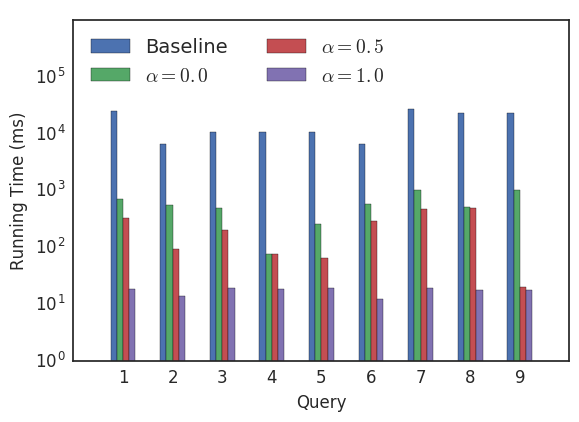
\includegraphics[width=\columnwidth]{figures/running_times_combined_bar.png}
\caption{Query runtimes with imputation on base tables, \ProjectName{}
    optimizing for quality ($\alpha=0$), and \ProjectName{} optimizing for
    performance ($\alpha=1$). Quality-optimized, on-the-fly imputation provides an order of
    magnitude speedup over imputing on base tables. Efficiency-optimized on-the-fly
    imputation can provide another order-of-magnitude speedup at the expense of quality. For
    relatively expensive queries over large datasets (Query 9), runtime of imputation can be reduced
    from~\acsbaseresulthours~to~\acsimputedbzeroresult.}
    
\label{fig:runtimes}
\end{figure}

%\Cref{fig:plantimes} provides a summary of the planning times for each of the queries.
%We exclude the planning time for queries that impute at base table, as that requires no
%planning. 

In the median query across a variety of queries and choices of $\alpha$, planning
constituted 8.5 percent of total runtime. In all cases, the optimizer
returned a query plan within 40ms, with times roughly constant between levels of $\alpha$.

% The one-standard-deviation
%intervals around the mean planning time often overlap, suggesting the planning component is
%constant in $\alpha$.

%\begin{figure}
%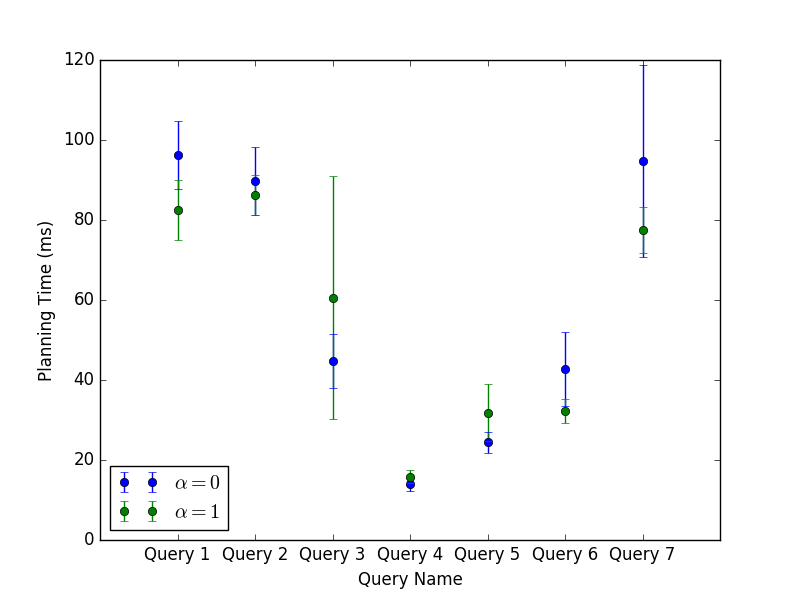
\includegraphics[width=\columnwidth]{figures/planning_times_imputedb.png}
%\caption{Planning times for each query}
%\label{fig:plantimes}
%\end{figure}

\subsubsection{Accuracy vs. Base-table Imputation}

\Cref{table:smape} shows the Symmetric-Mean-Absolute-Percentage-Error (SMAPE)\todo{cite SMAPE} for
\ProjectName{}'s query results when compared to running imputation on the base tables and
executing the query on this cleaned base data \cite{tofallis2015better}.  Each query was
separately run 200 times in both settings and then results from the two approaches were
paired up and compared tuple-wise.  We average tuple-wise absolute percentage deviations
within each iteration of a query, and we report this value averaged over all iterations.  We
can see that optimizing for quality indeed reduces the SMAPE of query results.  In general,
the SMAPE relative to the base-imputation approach are low in all cases --- between
\lowsmapealphazero{} and \highsmapealphaoneexacs{} percent ---, indicating that on-the-fly
imputation produces similar results to imputation at the base tables.

\begin{table}
\todo{extend this table to have counts with new results}
\centering
\begin{tabular}{rrr}
\toprule
 Query &  \textbackslashalpha &  SMAPE \\
\midrule
     0 &     0.0 &   0.47 \\
     0 &     1.0 &   0.15 \\
     1 &     0.0 &   0.28 \\
     1 &     1.0 &   0.40 \\
     2 &     0.0 &   0.00 \\
     2 &     1.0 &   0.00 \\
     3 &     0.0 &   0.03 \\
     3 &     1.0 &   0.22 \\
     4 &     0.0 &  11.18 \\
     4 &     1.0 &    NaN \\
     5 &     0.0 &   0.79 \\
     5 &     1.0 &   1.93 \\
     6 &     0.0 &   0.00 \\
     6 &     1.0 &   0.03 \\
     7 &     0.0 &   0.82 \\
     7 &     1.0 &  35.44 \\
     8 &     0.0 &   0.23 \\
     8 &     1.0 &   0.31 \\
     9 &     0.0 & 100.00 \\
     9 &     1.0 & 100.00 \\
\bottomrule
\end{tabular}

\caption{Symmetric-Mean-Absolute-Percentage-Error for queries run under different $\alpha$
    parameterizations relative to results when imputing on base table. Queries optimized for quality ($\alpha=0$) generally achieve
    lower error than queries optimized for efficiency ($\alpha=1$).}
\label{table:smape}
\end{table}

\subsubsection{Runtime of Base-table Imputation}
In many real-world cases, applying the imputation step at the base table is prohibitively
expensive.
To illustrate the increasing difficulty of such an approach as datasets scale, we ran the following query over the ACS dataset:
\begin{lstlisting}[breaklines]
SELECT AVG(c0) FROM acs_dirty;
\end{lstlisting}
Applying the imputation operation to the base table is extremely expensive, in our case
completing in \acsbaseresultminutes{} (\Cref{fig:runtimes}). In contrast, \ProjectName{} executes a quality-optimized version
in \acsimputedbzeroresult{} and a runtime-optimized version in \acsimputedboneresult{}. This highlights the potential
benefit of using our system for early data exploration.

For every imputation inserted into the query plan, a new statistical model is instantiated and trained before being used for imputation.
Although it is tempting to further optimize query execution in \ProjectName{} by pre-training imputation models while the analyst begins to make queries,
this is not desirable because the specific rows of data, set of complete attributes, and set of attributes to impute are not known until runtime.

\todobox{Jose: I'm not a fan of this line, I would remove}{Furthermore, at that point, it may make more sense to specify a coherent model over the entire base table instead.}

%%% Local Variables:
%%% mode: latex
%%% TeX-master: "main"
%%% End:

\section{Related Work}

There is related work in three primary areas: statistics, database research, and forecasting.

\subsection{Missing Values and Statistics}

Imputation of missing values is widely studied in the statistics and machine
learning communities. As highlighted in~\cite{gelman2006data}, missing data
can appear for a variety of reasons.
It can be missing uniformly at random or conditioned on
existing values (observed and missing). Methods in the statistical community
focus on correctly modeling relationships between attributes to account for different forms
of missingness. For example, \cite{burgette2010multiple} discuss the
usage of iterative decision trees for imputing missing data.

\cite{akande2015empirical} analyzes the performance of various
multiple imputation techniques on the American Community Survey dataset. 
The computational difficulties of imputing on large base
tables are well-known and can limit approaches. For example, \cite{akande2015empirical} finds that
one approach (MI-GLM) is prohibitively expensive when attempting to impute on data that
includes variables with potentially large domains (ten categories in their case).
In contrast, \ProjectName{} allows users to specify a trade-off between
imputation quality and runtime performance, allowing users to perform queries
directly on the entire dataset. Furthermore,
the query planner's imputation is guided by the requirements of each specific
query's operators, rather than requiring broad assumptions about query
workloads.  

\subsection{Missing Values and Databases}
There is a long history in the database community surrounding the
treatment of \nullv{}. As early as 1973,~\cite{codd1973understanding}
provided a treatment of the semantics of \nullv{}. Multiple
papers have described various (at times conflicting) treatments
of \nullv{}s~\cite{grant1977null}. \ProjectName's main design invariant---no relational operator
sees missing values for attributes it must operate on nor do users see
missing data---eliminates
the need to handle \nullv{} value semantics, while guaranteeing query evaluation soundness.

Database system developers and others have worked on techniques to automatically
detect dirty values, whether missing or otherwise, and rectify the errors if
possible. A survey of methods and systems is provided in~\cite{hellerstein2008quantitative}.

In~\cite{wolf2007query}, queries over databases with missing values are
processed directly using a statistical approach, taking advantage of correlations between
attributes. The tuples that match the original query as well as a ranking of
tuples with incomplete data that may match are returned. Our work differs in
that we allow any well-formed statistical technique to be used for imputation
and focus on returning results to the analyst as if the database had been
complete.

Designers of data stream processing systems frequently confront missing values
and consider them carefully in query processing. Often, if sensor error is the
cause of missing values, values can be imputed with high confidence. In~\cite{fernandez2009inter}, feedback punctuation is used to dynamically
reconfigure the query plan for state-dependent
optimizations as data continues to arrive. One of the applications of this framework is to avoid
expensive imputations as real-time conditions change. 
%We prove our
%algorithm and cost model produces an optimal set of plans to choose from,
%given the constraints of the search space.

Other work has looked at integrating statistical models into databases.
For example, BayesDB~\cite{mansinghka2015bayesdb} provides users with a simple interface to leverage statistical inference techniques in a database. Non-experts
can use a simple declarative language (an extension of SQL), to specify models
which allow missing value imputation, amongst other broader functionality.
Experts can further customize strategies and express domain knowledge to
improve performance and accuracy.

While BayesDB can be used for value imputation, this step is not framed
within the context of query planning, but rather as an explicit statistical
inference step within the query language, using the \verb|INFER| operation. 

BayesDB provides a great alternative for bridging the gap between
traditional databases and sophisticated modeling software. \ProjectName{}, in
contrast, aims to remain squarely in the database realm, while allowing
users to directly express queries on a potentially larger subset of their data.

\ProjectName's cost-based query planner 
is partially based on the seminal work developed for System R's query planning~\cite{blasgen1981system}.
However, in contrast to System R, \ProjectName{} performs additional optimizations for imputing missing data and
uses histogram transformations to account for the way relational and imputation operators affect the underlying
tuple distributions.

The planning algorithm that we present has similarities to the multi-objective query optimizer in~\cite{trummer2014}.
Both algorithms handle plans which have multiple cost functions by maintaining sets of Pareto optimal plans and pruning plans which become dominated.
In \ProjectName{}, costs are expected to grow monotonically as the size of the plan increases, which simplifies the optimization problem significantly.
\cite{trummer2014} handles the more complex case of cost functions which are piecewise linear, but not necessarily monotonic.

\subsection{Forecasting and Databases}
\cite{parisi2011embedding} introduce the idea of incorporating time-series forecast operators into
databases, along with the necessary relational algebra extensions. Their work explores the theoretical
properties of forecast operators and generalizes them into a family of operators, distinguished by
the type of predictions returned. They highlight the use of forecasting for replacing missing values.
In their follow on work~\cite{parisi2013temporal}, they identify various equivalence and containment
relationships when using forecast operators, which could be used to perform query plan transformations that guarantee the same result. They
explore forecast-first and forecast-last plans, which perform forecasting operations before and after executing all traditional
relational operators, respectively. 

\cite{fischer2013towards} describe the architecture of a DBMS with integrated forecasting operations for time-series, detailing
the abstractions necessary to do so.

In contrast to this work, \ProjectName{} is targeted at generic value imputation, not necessarily tailored to 
time-series. The optimizer is not based on equivalence transformations, nor are there guarantees of equal
results under different conditions. Instead, the optimizer allows users to pick their trade-off between
runtime cost and imputation quality. The search space considered by our optimizer is broader, not just
forecast-first/forecast-last plans, but rather imputation operators can be placed anywhere in the query plan
(with some restrictions). The novelty of our contribution lies in the successful incorporation of
imputation operations in non-trivial query plans with cost-based optimization.

\cite{duan2007processing} describes the Fa system and its declarative language for time-series forecasting. Their
system automatically searches the space of attribute combinations/transformations and statistical models
to produce forecasts within a given accuracy threshold. Accuracy estimates are determined using
standard techniques, such as cross-validation. 

Similarly to Fa, \ProjectName{} provides a declarative language, as
a subset of standard SQL.\@ \ProjectName{}, however, is not searching the space of possible
imputation models, but rather the space of query plans that incorporate imputation operators. Another major point
of distinction between \ProjectName{} and Fa is that the latter doesn't consider trade-offs between accuracy and computation time, but rather returns the most accurate forecast (with some stopping criterion).



%%% Local Variables:
%%% mode: latex
%%% TeX-master: "main"
%%% End:

\section{Conclusion}

As shown in \ProjectName{}, missing values and their imputation can successfully be integrated into the relational calculus and
existing plan optimization frameworks. We implement imputation actions, such as dropping or imputing values with a machine
learning technique, as operators in the algebra and use a simple, but effective, cost model to consider tradeoffs in 
information loss and time. In effect, user preferences for one or the other can be easily incorporated by adjusting a parameter.
Simple histogram transformations
provide incrementally updated cardinality estimates across operators in the plans, which allow us to provide more accurate cost estimates.
By taking a dynamic programming approach, we can consider a variety of operator placements
and input columns, while keeping planning tractable in real-world examples.

In our experiments, we considered a series of analytic queries (using relevant aggregates) and set queries (with simple projections) on real-world
American Community Survey data and synthetic data
and showed that the chosen query plan improves accuracy of results relative to simply ignoring missing values. Furthermore,
the variety of imputation operator placements across queries further emphasizes the lack of flexibility imposed by the coarse-grained
pre-processing approach to imputation. By allowing different imputation strategies for different queries, we
take a fine-grained approach to missing data, better addressing the often differing needs of database users.

We highlight the long history of dealing with missing data both in the statistical learning and database communities.
Similarly to existing work, we consider the impact of null values in databases and develop a simple set of invariants to 
successfully plan around them. In contrast to the statistical learning work, our emphasis is not on the specific algorithm
used to impute but rather on the timing of imputation in the execution of a query. In contrast to existing database work,
we incorporate imputation into a cost-based optimizer and hide any details
regarding missing values inside the system, allowing users to use traditional SQL and engage in normal workloads.

\subsection{Future Work}
\ProjectName{} opens up multiple avenues for further work. For instance, we
could extend our minimal/maximal imputation operators to consider global
information, such as the specific columns needed in operators higher up in the
query plan.  Our optimizer uses the same machine learning algorithm in all
instances of imputation operators. Integrating multiple possible algorithms
could allow for further fine-grained imputation, and honing the time complexity and
loss of these algorithms for an iterator model database could facilitate more
intelligent query plans and consistent interpretations of $\alpha$ across
strategies. For example, algorithms that learn in an online manner could
increase the efficiency of the system.  Furthermore, a multiple imputation
strategy could be followed for queries involving certain aggregates. Finally,
the underlying database for \ProjectName{} is far from a full-featured,
production database, so a natural step is to integrate imputation planning in a
widely-adopted production-quality database. This will likely expose further
opportunities for improvement.





%%% Local Variables:
%%% mode: latex
%%% TeX-master: "main"
%%% End:

\balance
\bibstyle{abbrv}
\printbibliography

\end{document}

%%% Local Variables:
%%% mode: latex
%%% TeX-master: t
%%% End:
